% !TEX root = ../Planning.tex
\section{Project description (D)}
\label{sec:project-description}

\subsection{The Ampersand project}
In November 2003, the Business Rules Manifesto\footnote{http://www.businessrulesgroup.org/brmanifesto.htm} was written, with the main purpose of declaring independence for business rules in the world of requirements.
The manifesto supports the vision of business rules as equivalent to requirements.
This is considered a radical change on how people see the world of business architecture.

Later on, the Ampersand approach was created as a way for defining business rules.
The approach puts the rules in the center, using them to define the business processes.
Ampersand is named after the \& symbol with the desire of realizing results for both business and IT, in an efficient and effective way.

In a series of research projects, the Ampersand software was created, improved and used in business and academic contexts.
The Ampersand end-users write business rules in a specific language, and compile that specification into functional specification, documentation and working software prototypes.
The theory behind Ampersand has been deeply studied, and is based on mathematical concepts e.g. Tarski's axioms.

\subsection{Current situation}


\subsection{Goal of the project}
The main objective for the graduation project is to implement useful feedback in the Ampersand parser.
If this task can be successfully accomplished, a list of open issues can be addressed by the project members.

\subsection{Project architecture, components and environment}
See figures~\ref{fig:architecture} and \ref{fig:data-flow}.

\begin{figure}[h]
  \centering
  \includegraphics[width=\textwidth]{Figures/ADL_systeemarchitectuur}
  \caption[Architecture of the project]{Architecture of the project, showing where the parser fits in the Ampersand system}
  \label{fig:architecture}
\end{figure}

\begin{figure}[h]
  \centering
  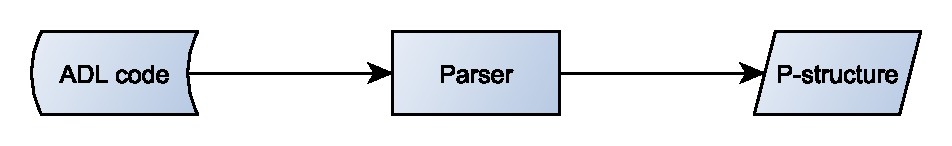
\includegraphics[width=0.5\textwidth]{Figures/Architecture}
  \caption{Relevant data flow for the Ampersand parsing component}
  \label{fig:data-flow}
\end{figure}

\subsection{Critical success factors}

\subsection{Our objectives and commitments towards the project and customer}
